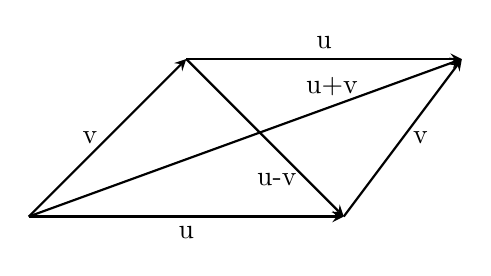
\begin{tikzpicture}
\coordinate(N1) at (-3.5,68)  ;
\coordinate(N2) at (-1.5,70) {} ;
\coordinate(N3) at (2,70) {}  ;
\coordinate(N4) at (0.5,68) {}  ;
\draw[-stealth,thick](N1)--node[pos=.5,left ] {v}(N2);
\draw[-stealth,thick](N2)--node[pos=.5,above ] {u}(N3);
\draw[-stealth,thick](N1)--node[pos=.5,below] {u}(N4);
\draw[-stealth,thick](N4)--node[pos=.5,right] {v}(N3);
\draw[-stealth,thick](N1)--node[pos=.7,above ] {u+v}(N3);
\draw[-stealth,thick](N2)--node[pos=.765, left] {u-v}(N4);
\end{tikzpicture}